%!TEX root = thesis.tex

\chapter{Introduction}
\label{chap:introduction}

\begin{chapquote}{Frederick Brooks, \textit{The Mythical Man-Month}}
``In spite of progress in restricting and simplifying the structures of software, they remain inherently unvisualizable, thus depriving the mind of some of its most powerful conceptual tools. This lack not only impedes the process of design within one mind, it severely hinders communication among minds.''
\end{chapquote}


%  Together these two concepts are foundational to culture. A recent push in hardware towards perfecting and simplifying design as a means to communicate intention more effectively has further blurred the lines between these two concepts. However, although the hardware industry has had a marked benefit from the combination of these two concepts, software process has largely missed out.

Introductions...\\
Art and understanding have long been associated.\\
-introduce the topic...\\

-introduce visualisations...\\
Software visualisations intend to communicate the software process more effectively.
-introduce live coding...\\
-suggest the problem statement and tie in the quote...\\
Live coding is a relatively new and developing field intending to further blur the lines between the worlds of art and understanding. Live coding provides exposure of the programming process to an audience, with the audience often having no background in programming.

As the complexity of software increases, better methods are required for communicating software structure, software changes and, perhaps most importantly, the need for communicating how the programmer performs the task of programming. Software visualisation has a long way to go in effectively communicating software but by visualising software...

% Live coding is a means of combining the artistic goal of enjoyment and the educational aspects associated with programming. However, due to the nature and maturity of live coding, these goals may be overlooked in the quest to improve the technical aspects of the live coding process.

This thesis investigates the proposition that ``code visualisation improves observer understanding and enjoyment'' in the setting of a live arts practice. More specifically, this thesis investigates the question ``can the application of visualisation techniques to live coding enhance audience experience by increasing understanding and enjoyment?''. These questions were examined through a process of prototype development, user study evaluation and refinement.\\

Definitions...\\
-define live coding, understanding and enjoyment\\
-define visualisation techniques\\
-define the programmer and observer relationship\\
-define audience experience\\

This thesis will explore the application of software visualisations to the process of live coding.
Introductory discussion/summary...\\
-this thesis will explore code visualisations\\
-specifically, it will investigate visuals within the combination of the domains of software and music\\
-will be using live coding as a platform and case study for this (will discuss later)\\
-will develop and test code visualisations on audiences with audiences of varied levels of experience with programming, addressing code comprehension\\


% -some useful quotes to be summarised somewhere... maybe here or in lit review\\
% ``Software is invisible and unvisualizable. Geometric abstractions are powerful tools. The floor plan of a building helps both architect and client evaluate spaces, traffic flows, views. Contradictions become obvious, omissions can be caught. Scale drawings of mechanical parts and stick-figure models of molecules, although abstractions, serve the same purpose. A geometric reality is captured in a geometric abstraction.''~\cite{Brooks1995}



% For most of its history source code has been displayed as simple text due to the expressiveness of this format and despite its inefficiencies. It is only recently, due to ever increasing programming language complexity and increasing computational power, that code annotations and syntax highlighting have become more commonplace. Nevertheless, these visual enhancements rarely provide information beyond the basic grammar of the language they are intended to augment. The limitations of this approach are becoming ever more apparent as programming languages and interactive programming environments move towards the need for real-time comprehension and a need to understand the source code within the context of a running program.\\


% Software engineering practice and art are often considered opposing ends of the spectrum. 

% This project will examine the relationship between aesthetics and educational aspects of code visualisiatons applied to two fields - an industry based application and a new media art application. 

% Questions:
% (1) What about the multimedia arts domain? What about the application of aesthetics and consideration for design within the space of software engineering? Both are widely accepted areas

% (2) Why don't we even have the most simple of tools to visualise changing code structure? Too complex? Not helpful? Why must code structures be designed statically?

% (3) Where is the future of programming? It is esentially the same as it was when it was first created. (Focus on higher abstractions in some fields? Move towards less abstraction...) Yet today it claims to be interactive/responsive etc...


\section{Background}

\subsection{History}

Discuss illustrations and the earliest representations of the world...

\begin{figure}
    \centering
    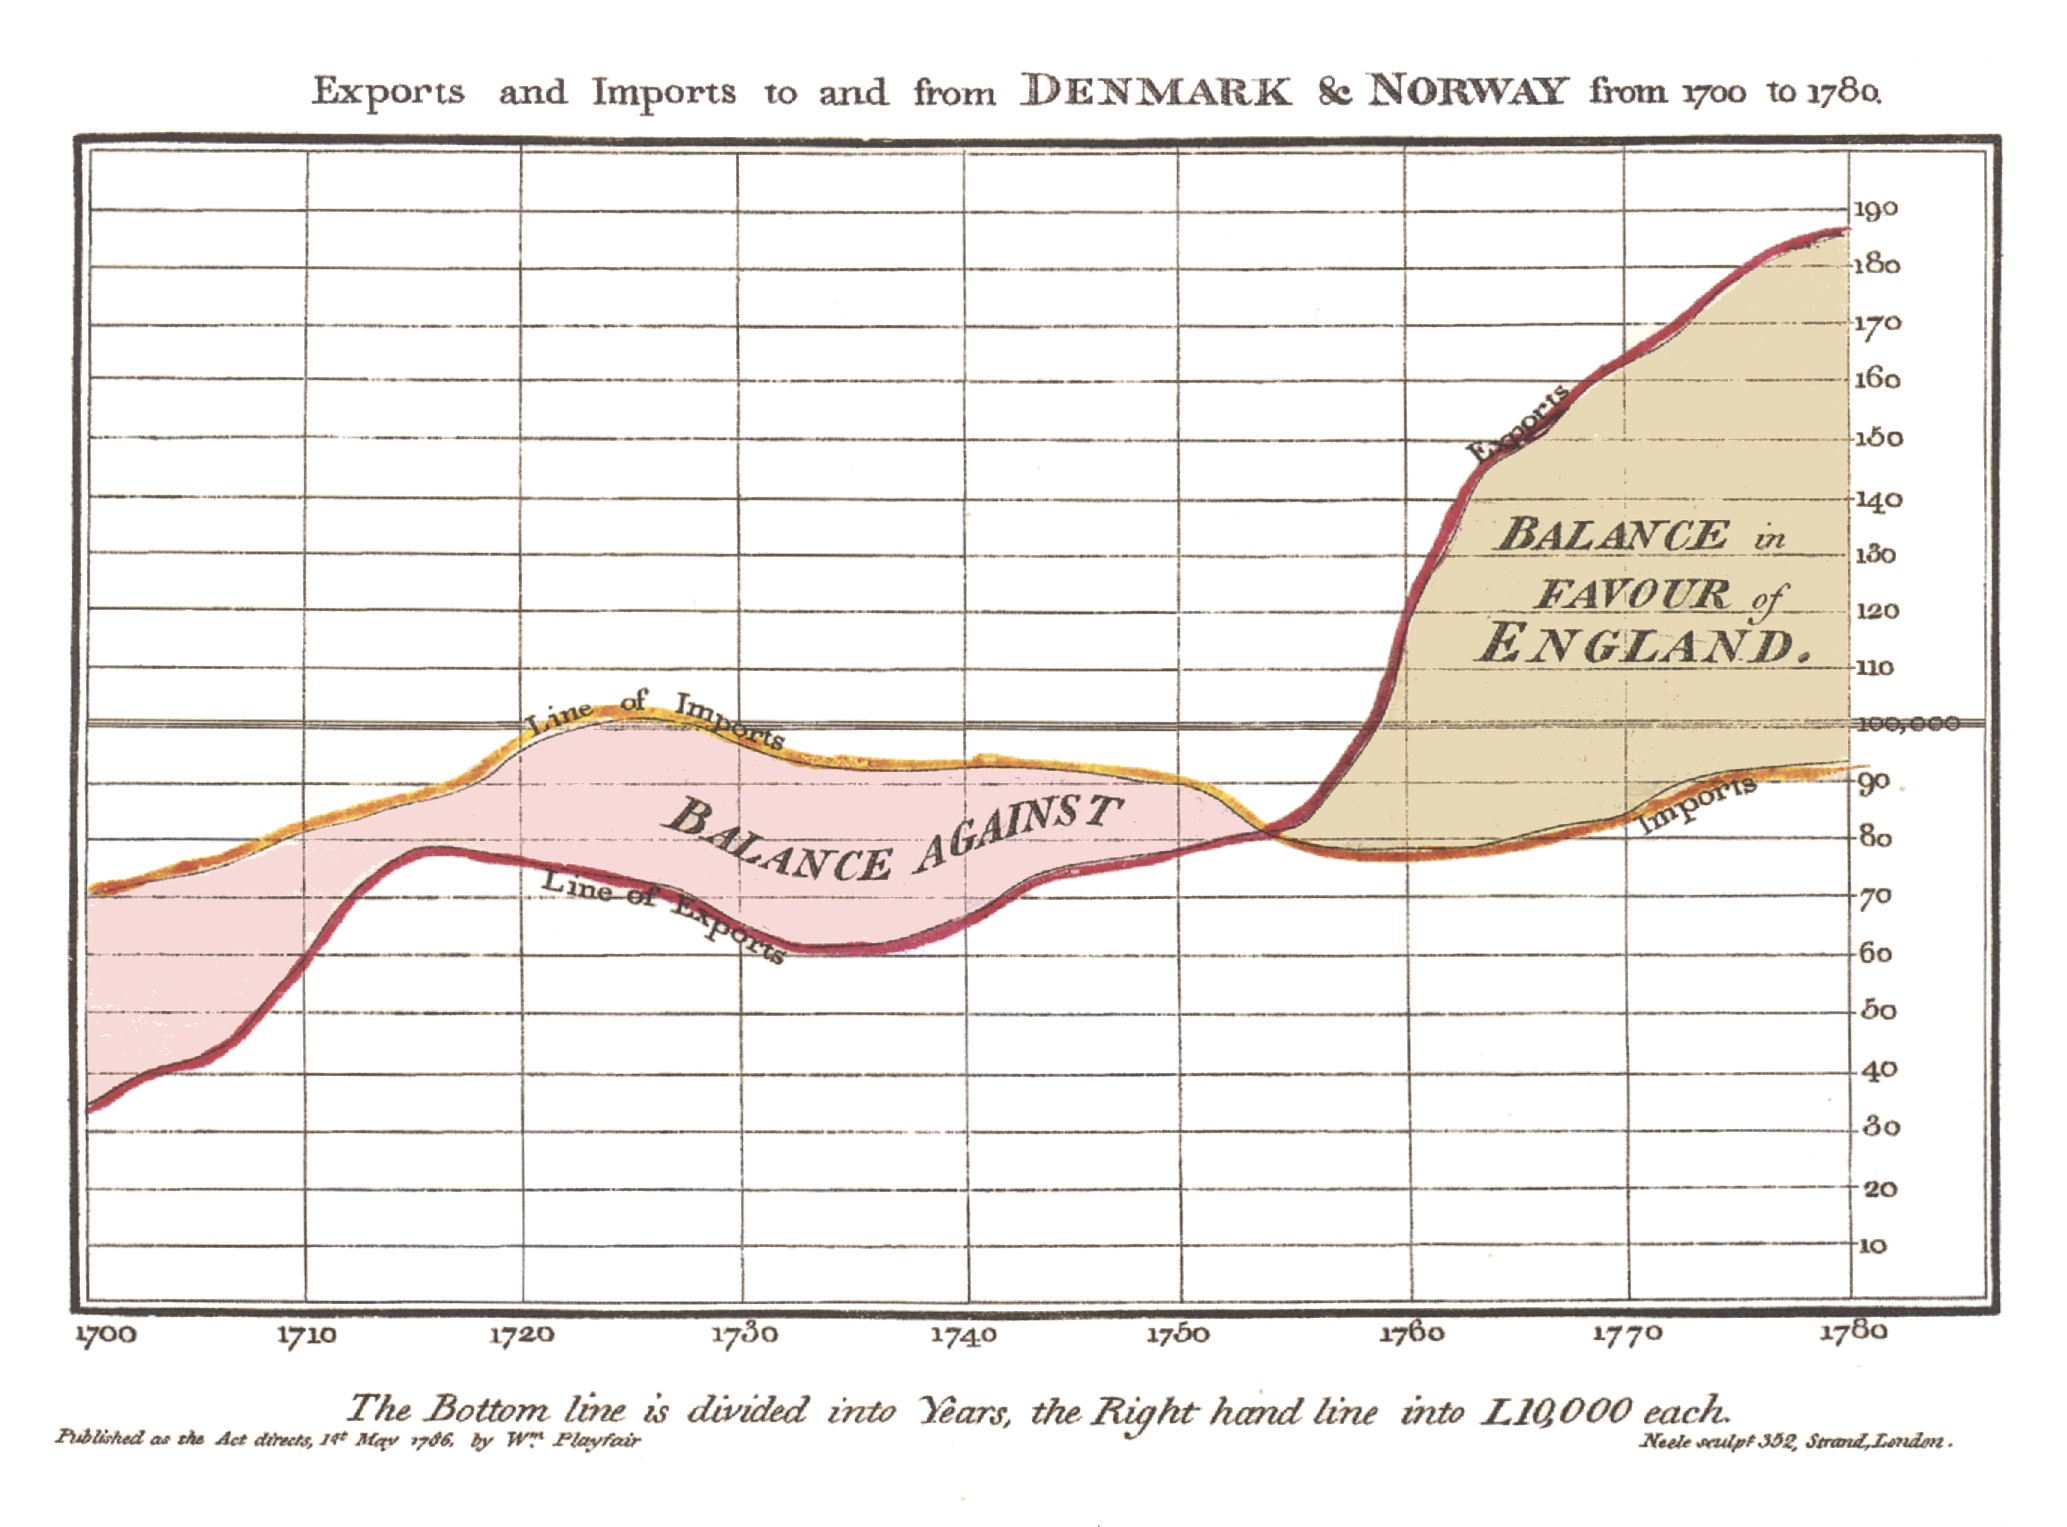
\includegraphics[width=0.8\textwidth]{../images/playfair-graph.png}
    \caption{An early example of visualisation showing the balance of trade between England versus Denmark and Norway from 1700 to 1780~\protect\cite{Playfair1786}.}
    \label{fig:playfair-graph}
\end{figure}

Since its inception, the visualisation of data has revolutionised how information is represented and understood. The earliest examples of visually summarising data through the use of visualisations occurred in William Playfair's \textit{The Commercial and Political Atlas}. Playfair developed a number of graphical representations of data that are very common today (see Figure~\ref{fig:playfair-graph} for an example) including the line chart, the bar chart and the pie chart.

Discuss progress to computation of data on computers and effect on the direction of visualisation...

Discuss information needs of the modern age...

\subsection{Visualisation}

Visualisation is the process of 

Animated visualisations...

A number of existing code visualisations show an interactive visualisation Existing code visualisations and representations...\\
-gource~\cite{Caudwell2010}\\
-code flower\\
-lighttable - inline feedback (developed due to the idea that code is unobservable, indirect and incidentally complex) \\
-code annotations~\cite{Swift2013}

\subsection{Live Coding}

Commercial sotware environments...
-code hotswapping
-etc...

Live coding...
-impact on the software development and scientific visualsation environment...

Some of the most important and influential live coding environments over the last decade have included SuperCollider~\cite{McCartney}, ChucK~\cite{Wang2008} and Extempore~\cite{Sorensen}. These environments have a growing following as the field of live coding matures.

\section{Structure}

A process of design iteration and evaluation was conducted. Three studies were administered, including one field studies and two laboratory studies.

The structure of this thesis consists of Chapter~\ref{chap:literature-review} summarising the literature including the basis for and the direction of this thesis. Following this, Chapter~\ref{chap:exploratory-field-study} discusses the initial exploratory field study conducted to investigate existing perception and understanding of the live coding process. Chapter~\ref{chap:visualisation-design} discusses the first iteration of the visualisation prototype developed following the results of the exploratory field study. Chapter~\ref{chap:user-study} summarises the first user study conducted with the visualisation prototype. Chapter~\ref{chap:visualisation-refinement} discusses refinement of the visualisation prototype motivated by the results of the first user study. Chapter~\ref{chap:follow-up-user-study} discusses the follow-up user study conducted to analyse the refined visualisations. Chapter~\ref{chap:summary} summarises the results of the user studies, contributions, limitations and future work. Finally, Chapter~\ref{chap:conclusion} provides some final words to conclude the thesis.




% -----------------------------------

% [from live coding paper]

% ``Show us your screens\ldots Code should be seen as well as heard'',
% declares the draft manifesto of ``TOPLAP''~\cite{Toplap}, an
% international organisation devoted to the artistic performance
% practice of ``live coding''. In live coding, computer code is written
% in front of a live audience to generate music and visuals in real
% time. The ``show us your screens'' rhetoric underscores the need for
% authenticity to distinguish this artform from similar (but non-live)
% computational arts practices.

% But what is the benefit of the live coder showing their screen? In a
% live coding performance, non-expert live coding audience members spend
% much of their time staring at raw (usually text-based) computer code.
% Until now, little empirical study has been undertaken to gauge an
% audience's understanding of that computer code and whether, from an
% audience perspective, code really should be ``seen as well as heard''.

% Traditional approaches to source code visualisation
% (see~\cite{Novais2013} for a review) often focus on structure of the
% source code (e.g. visualising complex object/class relationships)
% rather than the \emph{process} of programming. In a process-oriented
% activity such as live coding, different code visualisation techniques
% are necessary~\cite{McLean2010a,Magnusson2013}. However, these
% academic treatments of code visualisation in live coding adopt a
% survey-based approach, and the techniques discussed have not been
% subject to empirical evaluation.

% In this paper, we examine the audience's experience of the displayed
% code during live coding performances and to see whether code-driven
% visualisations might improve both the audience enjoyment and the
% audience understanding of these performances. This exploration takes
% place initially through the results of an exploratory field study at a
% contemporary arts festival, and subsequently through a lab-based
% follow-up user study.


% -----------------------
% Questions to ask (thesis post-mortem):

% What was your thesis about?
% What did you find out?

% -------------------

% didactic vs aesthetic
% industry vs art

% The purpose of software engineering is to bring together ideas from many fields into one - developing good software that is fit for purpose and fit for use. The systems engineering perspective of software engineering. However, one area where software engineering has had little influence and little influence has been taken from is the area of art.


% Often put on separate ends of the spectrum... unless you are building software for multimedia practice - even then though...


%%--------------------------------------------

% -code is often difficult to quickly understand
% -some observers may lack the experience to understand the software or the programming process

% Additionally, how we program does not achieve the goals we set out to achieve (from $https://www.youtube.com/watch?v=1f13TTu_X9k$, taken from presentation reimagining programming languages):
% -programming is unobservable (looking at the system through a keyhole)
% -programming is indirect (no direct feedback)
% -programming is incidentally complex (complexity not inherent in the problem that we need to solve)

%%--------------------------------------------

% -how can we improve source code comprehension?
% -how can we aid understanding of the programming process?
% -better yet, how can we better communicate the programmers intention?

% -techniques such as modelling or code documentation aren’t dynamic or flexible
% -don’t allow for close to realtime understanding
% -an effective technique is the use of visualisations
% -it would be valuable to use visualisations as a means to communicate the programmer’s intention

%%--------------------------------------------



